\documentclass[sigconf]{acmart}

\usepackage{tikz}
\usetikzlibrary{arrows.meta}

\usepackage{lineno}
\usepackage{isabelle,isabellesym}
\isabellestyle{tt}
\renewenvironment{isabelle}{%
  \bigbreak\noindent\hspace{\parindent}%
  \begin{minipage}{\textwidth-\parindent}% use minipage to prevent page breaks
  \begin{isabellebody}%
  \begin{tabbing}%
}{%
  \end{tabbing}%
  \end{isabellebody}%
  \end{minipage}%
  \bigbreak%
}
\renewcommand{\isacartoucheopen}{}
\renewcommand{\isacartoucheclose}{}

\setcopyright{rightsretained}
\copyrightyear{2019}
\acmYear{2019}
\acmDOI{}
\acmConference[]{}{}{}
\acmBooktitle{}
\acmPrice{}
\acmISBN{}

\begin{document}
\title{A highly-available move operation for replicated trees}

\author{Martin Kleppmann}
\email{mk428@cl.cam.ac.uk}
\orcid{0000-0001-7252-6958}
\affiliation{%
  \institution{Department of Computer Science and Technology}
  \streetaddress{15 JJ Thomson Avenue}
  \city{Cambridge}
  \state{}
  \postcode{CB3 0FD}
  \country{United Kingdom}
}

\author{Dominic P.\ Mulligan}
\email{Dominic.Mulligan@arm.com}
\orcid{0000-0003-4643-3541}
\affiliation{%
  \institution{Arm Research}
  \streetaddress{110 Fulbourn Road}
  \city{Cambridge}
  \state{}
  \postcode{CB1 9NJ}
  \country{United Kingdom}
}

\author{Victor B.\ F.\ Gomes}
\email{vb358@cl.cam.ac.uk}
\orcid{0000-0002-2954-4648}
\affiliation{%
  \institution{Department of Computer Science and Technology}
  \streetaddress{15 JJ Thomson Avenue}
  \city{Cambridge}
  \state{}
  \postcode{CB3 0FD}
  \country{United Kingdom}
}

\author{Alastair R.\ Beresford}
\email{arb33@cl.cam.ac.uk}
\orcid{0000-0003-0818-6535}
\affiliation{%
  \institution{Department of Computer Science and Technology}
  \streetaddress{15 JJ Thomson Avenue}
  \city{Cambridge}
  \state{}
  \postcode{CB3 0FD}
  \country{United Kingdom}
}

%\renewcommand{\shortauthors}{Kleppmann, Mulligan, Gomes, and Beresford}

\begin{abstract}
    TODO abstract.
\end{abstract}
\maketitle

\section{Introduction}\label{sec:intro}

For many systems and applications, the data model that describes the system state is a tree.
For example:
\begin{itemize}
    \item Most \textbf{filesystems}, e.g. on Windows and Unix-like OSes, are organised as a tree: folders or directories are branch nodes, and files are leaf nodes.\footnote{In filesystems that support hardlinks, the structure is---strictly speaking---a restricted DAG in which a file inode can be referenced from multiple places in the directory tree, but directories cannot have more than one parent directory.
        However, for the purposes of this paper, we will treat a filesystem as a tree; given such a tree, it is easy to add hardlinks and symlinks as features on top.}
        In Unix-style filesystems, the nodes of the tree are known as \emph{inodes}.
    \item \textbf{Rich text editors} maintain a tree of textual structures such as paragraphs, bulleted and numbered lists, figures, sections, and so on.
        These can be nested inside each other: for example, a paragraph may appear inside a bullet point of a bulleted list, which may in turn appear inside a numbered point of an enumeration.
        Rich text documents are typically represented in memory using the Document Object Model (DOM), and written to file in HTML, XML, or JSON format.
    \item \textbf{Vector graphics} and \textbf{presentation software} represents images using graphical objects such as text boxes, rectangles, ellipses, lines, and so on.
        These objects are contained within nodes representing pages of a document, or slides of a presentation.
        Multiple objects may be combined into a \emph{group} so that they can be manipulated as a unit; this corresponds to making these objects children of a common parent node.
        Multiple objects and groups may in turn be combined into higher-level groups, forming a tree.
        %Moreover, the order of nodes determines visibility (i.e.\ objects that are ``further back'' may be obscured by objects that are ``closer to the front'').
    \item Personal \textbf{note-taking} and \textbf{task-management tools} such as Org-mode for Emacs~\cite{OrgMode} or OmniOutliner~\cite{OmniOutliner} explicitly present the user with a tree structure that they can inspect and manipulate.
\end{itemize}

In this paper we consider applications that use such a tree data model, and that replicate this tree across multiple replicas.
Moreover, we focus on \emph{optimistic replication}~\cite{Saito:2005jw}, that is, systems in which any replica can autonomously make changes to the data, without waiting for communication or coordination with any other replicas.
Such systems have the advantage that they can continue processing read and write requests even in the presence of arbitrary network partitions; in other words, they are \emph{available} and \emph{partition-tolerant} in the sense of the CAP theorem~\cite{Gilbert:2002il}.
This approach is desirable since it enables disconnected operation in a mobile computing context, and high availability in geo-replicated settings.

As the tree structure may be concurrently modified on different replicas, the state of these replicas may temporarily diverge.
In this paper we show how the replicas can nevertheless achieve \emph{strong eventual consistency}~\cite{Shapiro:2011un}: as the replicas communicate, we guarantee that they will converge towards a consistent state.
Our algorithm for achieving convergence is an example of a \emph{Conflict-free Replicated Data Type} or CRDT~\cite{Shapiro:2011wy,Shapiro:2011un}.

In this paper we use an abstract model of a tree that can support any of the applications listed above, including distributed filesystems.
We allow replicas to manipulate this tree in any way: by creating new nodes, deleting nodes, or moving subtrees to a new location within the tree.
While there are many existing systems that support creating and deleting nodes (see Section~\ref{sec:relwork}), the key innovation of our algorithm is the support for moving subtrees.
We explain in Section~\ref{sec:move-is-hard} why this move operation is so challenging.

Our contributions in this work are as follows:
\begin{itemize}
    \item We define a Conflict-free Replicated Data Type for trees that supports a \emph{move} operation, without requiring any coordination between replicas such as locking or consensus.
        As discussed in Section~\ref{sec:impossibility}, this has previously been thought to be impossible to achieve \cite{Najafzadeh:2017vk,Najafzadeh:2018bw}.
    \item We formalise our algorithm using Isabelle/HOL~\cite{DBLP:conf/tphol/WenzelPN08}, an interactive proof assistant, and produce a computer-checked proof of correctness of our algorithm.
        In particular, we prove that arbitrary concurrent modifications to the tree can be merged such that all replicas converge towards a consistent state (strong eventual consistency).
    \item To demonstrate the practical viability of the algorithm we extract a formally verified, executable implementation from the Isabelle/HOL definitions, and perform tests on this implementation.
    \item We perform experiments with replicated filesystem products such as Dropbox and Google Drive, and show that they exhibit problems that would be prevented by our algorithm.
\end{itemize}

\begin{figure*}
\centering
\begin{tikzpicture}
  \tikzstyle{time}=[thick,->,gray]
  \tikzstyle{network}=[thick,dashed,blue,-{Stealth[length=3mm]}]
  \node [anchor=east] at (-1.8,3) {Replica 1:};
  \node [anchor=east] at (-1.8,0) {Replica 2:};
  \node [rectangle,draw] (start1) at (0,3) {
      \begin{tikzpicture}[level distance=7mm]
          \tikzstyle{level 1}=[sibling distance=10mm]
          \tikzstyle{level 2}=[sibling distance=6mm]
          \node {$\mathsf{root}$}
              child {node {$A$} child {node {$a_1$}} child {node {$a_2$}} child {node {$a_3$}}}
              child {node {$B$}}
              child {node {$C$}};
      \end{tikzpicture}
  };
  \node [rectangle,draw] (start2) at (0,0) {
      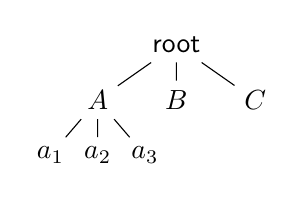
\begin{tikzpicture}[level distance=7mm]
          \tikzstyle{level 1}=[sibling distance=10mm]
          \tikzstyle{level 2}=[sibling distance=6mm]
          \node {$\mathsf{root}$}
              child {node {$A$} child {node {$a_1$}} child {node {$a_2$}} child {node {$a_3$}}}
              child {node {$B$}}
              child {node {$C$}};
      \end{tikzpicture}
  };
  \node [rectangle,draw] (change1) at (5,3) {
      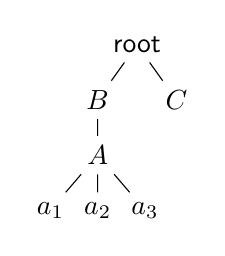
\begin{tikzpicture}[level distance=7mm]
          \tikzstyle{level 1}=[sibling distance=10mm]
          \tikzstyle{level 3}=[sibling distance=6mm]
          \node {$\mathsf{root}$}
              child {node {$B$} child {node {$A$} child {node {$a_1$}} child {node {$a_2$}} child {node {$a_3$}}}}
              child {node {$C$}};
      \end{tikzpicture}
  };
  \node [rectangle,draw] (change2) at (5,0) {
      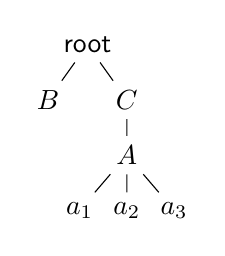
\begin{tikzpicture}[level distance=7mm]
          \tikzstyle{level 1}=[sibling distance=10mm]
          \tikzstyle{level 3}=[sibling distance=6mm]
          \node {$\mathsf{root}$}
              child {node {$B$}}
              child {node {$C$} child {node {$A$} child {node {$a_1$}} child {node {$a_2$}} child {node {$a_3$}}}};
      \end{tikzpicture}
  };
  \node [rectangle,draw,inner sep=3mm] (merge1) at (8.2,3) {?};
  \node [rectangle,draw,inner sep=3mm] (merge2) at (8.2,0) {?};
  \draw [time] (start1.east) -- node [above,text width=2.5cm,text centered,inner ysep=5pt] {Move $A$ to be a child of $B$} (change1.west);
  \draw [time] (change1.east) -- (merge1.west);
  \draw [time] (start2.east) -- node [above,text width=2.5cm,text centered,inner ysep=5pt] {Move $A$ to be a child of $C$} (change2.west);
  \draw [time] (change2.east) -- (merge2.west);
  \draw [network] (6.5,0) to [out=90,in=270] (7.2,3);
  \draw [network] (6.5,3) to [out=270,in=90] (7.2,0);
  \node [rotate=90,blue,font=\footnotesize] at (7.5,1.5) {network communication};
  \path [draw,dotted] (-3.1,1.5) -- (8.7,1.5);
  %%%
  \node [fill=red!15] at (9.83,4.10) {(\emph{a})};
  \node [fill=red!15] at (14.18,4.10) {(\emph{b})};
  \node [fill=red!15] at (9.84,1.10) {(\emph{c})};
  \node [fill=red!15] at (14.15,1.10) {(\emph{d})};
  \node [rectangle,draw] at (10.9,3) {
      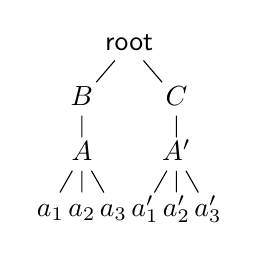
\begin{tikzpicture}[level distance=7mm]
          \tikzstyle{every node}=[text height=5pt,text depth=0pt]
          \tikzstyle{level 1}=[sibling distance=12mm]
          \tikzstyle{level 3}=[sibling distance=4mm]
          \node {$\mathsf{root}$}
              child {node {$B$} child {node {$A$} child {node {$a_1$}} child {node {$a_2$}} child {node {$a_3$}}}}
              child {node {$C$} child {node {$A'$} child {node {$a_1'$}} child {node {$a_2'$}} child {node {$a_3'$}}}};
      \end{tikzpicture}
  };
  \node [rectangle,draw] at (13.5,3) {
      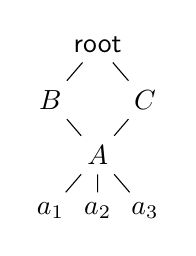
\begin{tikzpicture}[level distance=7mm]
          \tikzstyle{level 1}=[sibling distance=12mm]
          \node at (0,1.4) {$\mathsf{root}$} child {node (b) {$B$}} child {node (c) {$C$}};
          \tikzstyle{level 1}=[sibling distance=6mm]
          \node (a) at (0,0) {$A$} child {node {$a_1$}} child {node {$a_2$}} child {node {$a_3$}};
          \draw (b) -- (a);
          \draw (c) -- (a);
      \end{tikzpicture}
  };
  \node [rectangle,draw] at (10.7,0) {
      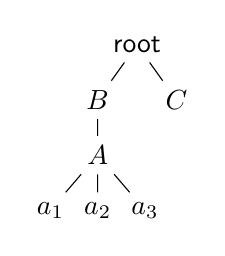
\begin{tikzpicture}[level distance=7mm]
          \tikzstyle{level 1}=[sibling distance=10mm]
          \tikzstyle{level 3}=[sibling distance=6mm]
          \node {$\mathsf{root}$}
              child {node {$B$} child {node {$A$} child {node {$a_1$}} child {node {$a_2$}} child {node {$a_3$}}}}
              child {node {$C$}};
      \end{tikzpicture}
  };
  \node [rectangle,draw] at (13.3,0) {
      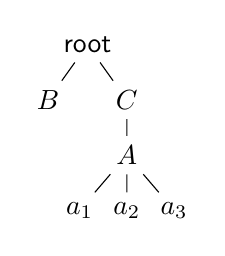
\begin{tikzpicture}[level distance=7mm]
          \tikzstyle{level 1}=[sibling distance=10mm]
          \tikzstyle{level 3}=[sibling distance=6mm]
          \node {$\mathsf{root}$}
              child {node {$B$}}
              child {node {$C$} child {node {$A$} child {node {$a_1$}} child {node {$a_2$}} child {node {$a_3$}}}};
      \end{tikzpicture}
  };
\end{tikzpicture}
\caption{Replica 1 moves $A$ to be a child of $B$, while concurrently replica 2 moves the same node $A$ to be a child of $C$. Boxes (\emph{a}) to (\emph{d}) show possible outcomes after the replicas have communicated and merged their states.}
\label{fig:move-same-item}
\Description{}
\end{figure*}

\begin{figure*}
\centering
\begin{tikzpicture}
  \tikzstyle{time}=[thick,->,gray]
  \tikzstyle{network}=[thick,dashed,blue,-{Stealth[length=3mm]}]
  \node [anchor=east] at (-1.2,3) {Replica 1:};
  \node [anchor=east] at (-1.2,0) {Replica 2:};
  \node [rectangle,draw] (start1) at (0,3) {
      \begin{tikzpicture}[level distance=7mm]
      \node {$\mathsf{root}$} child {node {$A$} child {node {$C$}}} child {node {$B$}};
      \end{tikzpicture}
  };
  \node [rectangle,draw] (start2) at (0,0) {
      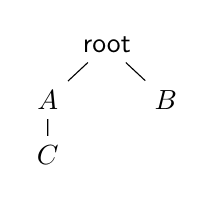
\begin{tikzpicture}[level distance=7mm]
      \node {$\mathsf{root}$} child {node {$A$} child {node {$C$}}} child {node {$B$}};
      \end{tikzpicture}
  };
  \node [rectangle,draw] (change1) at (4.5,3) {
      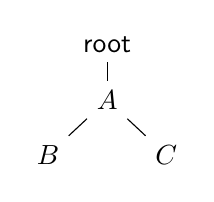
\begin{tikzpicture}[level distance=7mm]
      \node {$\mathsf{root}$} child {node {$A$} child {node {$B$}} child {node {$C$}}};
      \end{tikzpicture}
  };
  \node [rectangle,draw] (change2) at (4.5,0) {
      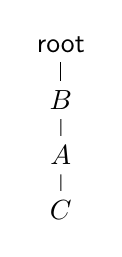
\begin{tikzpicture}[level distance=7mm]
      \node {$\mathsf{root}$} child {node {$B$} child {node {$A$} child {node {$C$}}}};
      \end{tikzpicture}
  };
  \node [rectangle,draw,inner sep=3mm] (merge1) at (8,3) {?};
  \node [rectangle,draw,inner sep=3mm] (merge2) at (8,0) {?};
  \draw [time] (start1.east) -- node [above,text width=2.5cm,text centered,inner ysep=5pt] {Move $B$ to be a child of $A$} (change1.west);
  \draw [time] (change1.east) -- (merge1.west);
  \draw [time] (start2.east) -- node [above,text width=2.5cm,text centered,inner ysep=5pt] {Move $A$ to be a child of $B$} (change2.west);
  \draw [time] (change2.east) -- (merge2.west);
  \draw [network] (6.0,0) to [out=90,in=270] (6.7,3);
  \draw [network] (6.0,3) to [out=270,in=90] (6.7,0);
  \node [rotate=90,blue,font=\footnotesize] at (7.0,1.5) {network communication};
  \path [draw,dotted] (-2.5,1.6) -- (8.5,1.6);
  %%%%%
  \node [rectangle,draw] at (10.95,3) {
      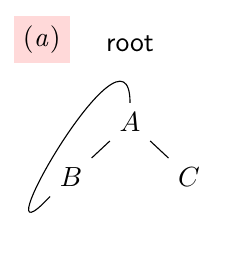
\begin{tikzpicture}[level distance=7mm]
      \useasboundingbox (-1.3,-1.3) rectangle (1,1.2);
      \node [fill=red!15] at (-1.12,1.05) {(\emph{a})};
      \node at (0,1) {$\mathsf{root}$};
      \node (a1) {$A$} child {node (b1) {$B$}} child {node {$C$}};
      \draw (b1.south west) .. controls (-2,-2) and (0,1.5) .. (a1.north);
      \end{tikzpicture}
  };
  \node [rectangle,draw] at (13.8,3) {
      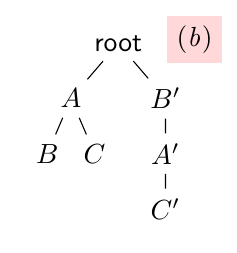
\begin{tikzpicture}[level distance=7mm]
      \useasboundingbox (-1.15,-2.3) rectangle (1.15,0.2);
      \node [fill=red!15] at (0.97,0.05) {(\emph{b})};
      \tikzstyle{level 1}=[sibling distance=12mm]
      \tikzstyle{level 2}=[sibling distance=6mm]
      \node {$\mathsf{root}$}
          child {node {$A$} child {node {$B$}} child {node {$C$}}}
          child {node {$B'$} child {node {$A'$} child {node {$C'$}}}};
      \end{tikzpicture}
  };
  \node [rectangle,draw] (start) at (10.95,0) {
      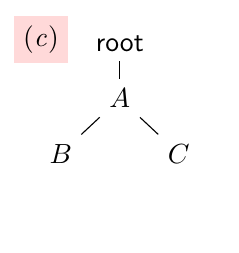
\begin{tikzpicture}[level distance=7mm]
      \useasboundingbox (-1.17,-2.3) rectangle (1.15,0.2);
      \node [fill=red!15] at (-1.00,0.05) {(\emph{c})};
      \node {$\mathsf{root}$} child {node {$A$} child {node {$B$}} child {node {$C$}}};
      \end{tikzpicture}
  };
  \node [rectangle,draw] (right) at (13.8,0) {
      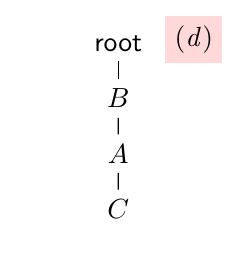
\begin{tikzpicture}[level distance=7mm]
      \useasboundingbox (-1.15,-2.3) rectangle (1.15,0.2);
      \node [fill=red!15] at (0.96,0.05) {(\emph{d})};
      \node {$\mathsf{root}$} child {node {$B$} child {node {$A$} child {node {$C$}}}};
      \end{tikzpicture}
  };
\end{tikzpicture}
\caption{Initially, nodes $A$ and $B$ are siblings. Replica 1 moves $B$ to be a child of $A$, while concurrently replica 2 moves $A$ to be a child of $B$. Boxes (\emph{a}) to (\emph{d}) show possible outcomes after the replicas have communicated and merged their states.}\label{fig:move-cycle}
\Description{Visualisation of trees with concurrent move operations}
\end{figure*}

\begin{figure*}
  \centering
  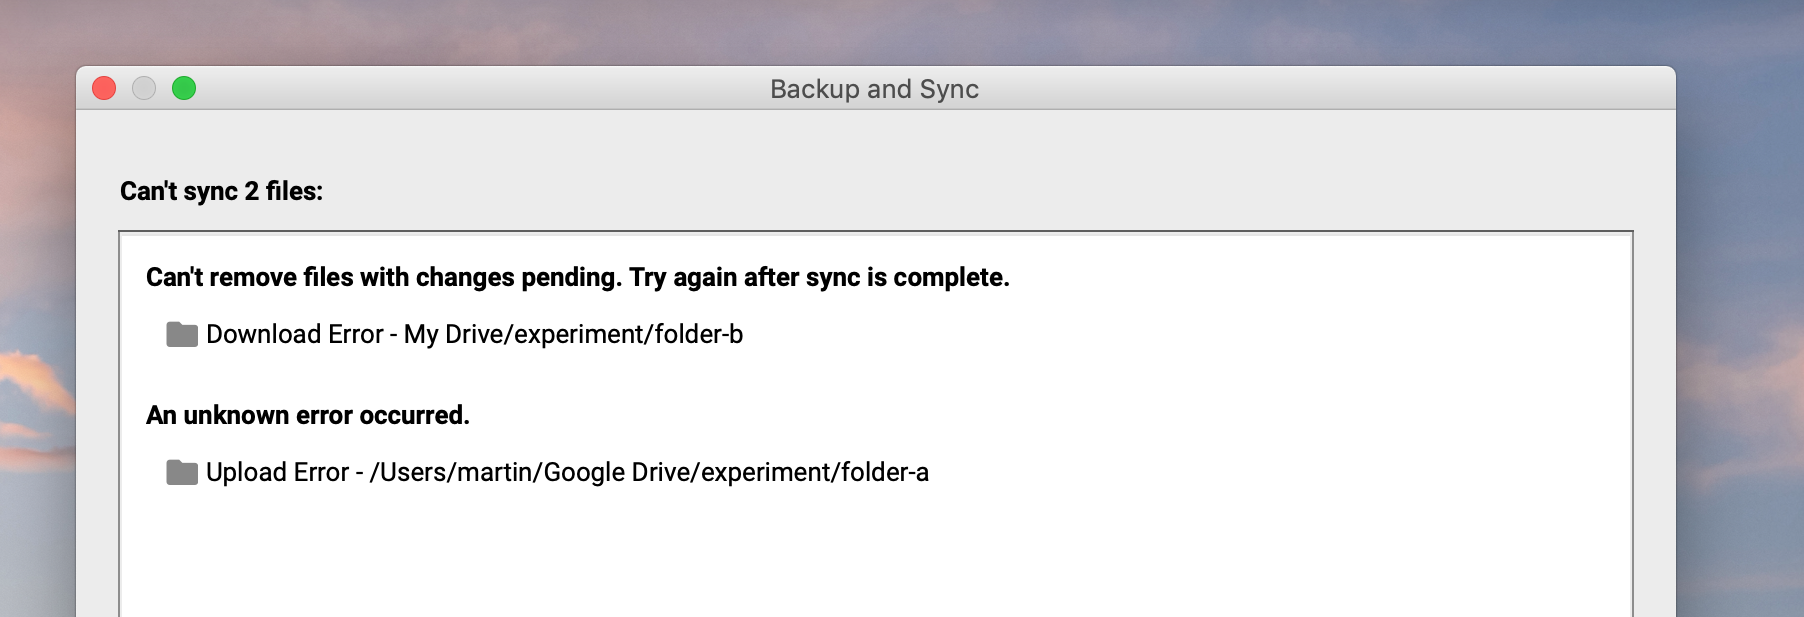
\includegraphics[width=\textwidth,keepaspectratio=true]{gdrive-error.png}
  \caption{Error message produced by Google Drive Backup and Sync on Mac OS as a result of performing the operations shown in Figure~\ref{fig:move-cycle}.}
  \label{fig:gdrive-error}
  \Description{Screenshot showing the errors ``Can't remove files with changes pending. Try again after sync is complete.'' and ``An unknown error occurred.''}
\end{figure*}

\section{Why a move operation is hard}\label{sec:move-is-hard}

Applications that rely on a tree data model often need to move a node from one location to another location within the tree, whereby all children of the moved node move along with it.
For example:
\begin{itemize}
    \item In a filesystem, any file or directory can be moved to a different parent directory.
        Moreover, renaming a file or directory is equivalent to moving it to a new name without changing its parent directory.
    \item In a rich text editor, a paragraph node can be turned into a bullet point.
        In the DOM tree this corresponds to creating a new bullet list node, creating a new bullet point node within it, and then moving the paragraph node to be a child of the new bullet point node.
    \item In presentation software, grouping two graphical objects corresponds to creating a new group node, and then moving the two objects to be children of the new group node.
\end{itemize}
As these operations are so common, it is not obvious why a move operation should be difficult in a replicated setting.
In this section we demonstrate by example some of the problems that arise with replicated trees, before proceeding to our solution in Section~\ref{sec:algorithm}.

\subsection{Concurrent moves of the same node}\label{sec:move-same-item}

The first difficulty arises when a node is moved to a new location on one replica, and concurrently the same node is moved to a different location on a different replica.
This scenario is illustrated in Figure~\ref{fig:move-same-item}, where replica 1 moves node $A$ to be a child of $B$, while concurrently replica 2 moves $A$ to be a child of $C$.
After the replicas communicate these operations to each other, what should the merged state of the tree be?

If a move operation is implemented by deleting the moved subtree from its old location, and then re-creating it at the new location, the merged state will be as shown in Figure~\ref{fig:move-same-item}a: the concurrent moves will duplicate the moved subtree, since each concurrent move independently recreates the subtree in each destination location.
We believe that this duplication is undesirable, since subsequent edits to nodes in the duplicated subtree will apply to only one of the copies.
Two users who believe they are collaborating on the same file may in fact be editing two different copies, which will then become inconsistent with each other.

Rather than duplicating the moved subtree, another possible resolution is for the destination locations of both moves to refer to the same node, as shown in Figure~\ref{fig:move-same-item}b.
However, the result is a DAG, not a tree.
POSIX filesystems to not allow this outcome, since they allow hardlinks only to files, but not to directories.

In our opinion, the only reasonable outcomes are those shown in Figure~\ref{fig:move-same-item}c and~\ref{fig:move-same-item}d: the moved subtree appears either in replica 1's destination location or in replica 2's destination location, but not in both.
Which one of these two is picked is arbitrary, due to the symmetry between the two replicas.
For example, the ``winning'' location could be picked based on a timestamp in the operations, similarly to the ``last writer wins'' conflict resolution method of Thomas's write rule~\cite{Johnson:1975we}.
All replicas pick the same operation as winner, and effectively ignore the conflicting operation.

We tested this scenario with file sync products Dropbox and Google Drive by concurrently moving the same directory to two different destination directories.\footnote{Experiment setup: we installed the official Mac OS clients for Dropbox and Google Drive on two computers, and configured them to each sync a directory on the local filesystem with the corresponding cloud service.
To test concurrent operations, we turned off the network interface on both computers, performed a move operation on the local filesystem of each computer, then reconnected both computers to the Internet and waited for them to sync.}
Dropbox exhibited the undesirable duplication behaviour of Figure~\ref{fig:move-same-item}a, while the outcome on Google Drive was as in Figure~\ref{fig:move-same-item}c/d.

\subsection{Moving a node to be a descendant of itself}\label{sec:move-cycle}

On a filesystem, the destination directory of a move operation must not be a subdirectory of the directory being moved.
For example, if \texttt{b} is a subdirectory of \texttt{a}, then the Unix shell command \texttt{mv a a/b/} will fail with an error.
This restriction is required because allowing this operation would introduce a cycle into the directory graph, and so the filesystem would no longer be a tree.
The same restriction is required in any other tree structure that supports a move operation.

In an unreplicated tree it is easy to prevent cycles being introduced: if the node being moved is an ancestor of the destination node, then the move operation must be rejected.
However, in a replicated setting a new problem arises: different replicas may perform operations that individually are safe, but whose combination leads to a cycle.

One example of such a scenario is illustrated in Figure~\ref{fig:move-cycle}.
Here, replica 1 moves $B$ to be a child of $A$, while concurrently replica 2 moves $A$ to be a child of $B$.
As each replica propagates its operation to the other replica, a careless implementation might end up in the state shown in Figure~\ref{fig:move-cycle}a, in which $A$ and $B$ have become locked in a cycle and detached from the tree.

Another possible resolution is shown in Figure~\ref{fig:move-cycle}b: the nodes involved in the concurrent moves (and their children) could be duplicated, so that both ``$A$ as a child of $B$'' and ``$B$ as a child of $A$'' can exist in the tree.
However, such duplication is undesirable for the same reasons as in Section~\ref{sec:move-same-item}.

In our opinion, the best way of handling the conflicting operations of Figure~\ref{fig:move-cycle} is to choose either Figure~\ref{fig:move-cycle}c or~\ref{fig:move-cycle}d: that is, either the result of applying replica 1's operation and ignoring replica 2's operation, or vice versa.
Like in Section~\ref{sec:move-same-item}, the winning operation can be picked based on an operation timestamp.

As before, we tested this scenario with Google Drive and Dropbox.
In Google Drive, one replica was able to successfully sync with the server, while the other replica displayed the ``unknown error'' message shown in Figure~\ref{fig:gdrive-error}.
The replica in error state refused to sync the conflicting directory, and its filesystem state remained inconsistent with the other replica.
This error state persisted until the directories on the erroring replica were manually moved to match the state of the other replica.

On the other hand, Dropbox exhibits the duplication behaviour shown in Figure~\ref{fig:move-cycle}b.

\subsection{The impossibility of a highly-available move operation}\label{sec:impossibility}

Najafzadeh et al.~\cite{Najafzadeh:2017vk,Najafzadeh:2018bw} have previously implemented a replicated filesystem with a move operation, and analysed the case of concurrent move operations introducing a cycle, as in Section~\ref{sec:move-cycle}.
Using the CISE ('Cause I'm Strong Enough) proof tool~\cite{DBLP:conf/popl/GotsmanYFNS16,Najafzadeh:2016fi} the authors confirm that it is not sufficient for the replica that generates a move operation to check whether the operation introduces a cycle: like in Figure~\ref{fig:move-cycle}, two concurrent operations may be safe individually, but introduce a cycle when combined.

Najafzadeh et al. propose two solutions to this problem: either to duplicate tree nodes, as in Figure~\ref{fig:move-cycle}b, or to execute a synchronous locking protocol that prevents two move operations concurrently modifying the same part of the tree.
The downside of a locking protocol is that the move operation is no longer highly available in the presence of network partitions, since it must wait for communication with other replicas.

While these solutions are valid, the authors go on to claim that these are the only possible options, asserting that ``no file system can support an unsynchronised move without anomalies, such as loss or duplication''~\cite{Najafzadeh:2018bw}.
We revise that claim in this paper: our algorithm does not perform any locking, coordination or synchronisation among replicas, but it nevertheless ensures that the tree invariants are always satisified (in particular, it never introduces cycles), and it never duplicates any tree nodes.
To our knowledge, our algorithm is the first to provide all of these properties simultaneously.
We give a precise specification of our algorithm's consistency properties in Section~\ref{sec:proof}.

\section{The replicated move operation}\label{sec:algorithm}

% - No Synchronisation or consensus required. Available in the sense of CAP
% - Rely only on uniqueness of node IDs, e.g. inode numbers
% - Composing JSON/XML tree by using list datatype
% - Location is Lww register. Concurrent move does not duplicate
% - Isabelle: combines the conciseness of pseudocode with the precision of mathematical notation.
% - Unlike NFS, can work offline 
% - Garbage collection: discard causally stable prefix


\begin{figure*}
\raggedright
\begin{isabellebody}
\internallinenumbers
\isacommand{datatype}\isamarkupfalse%
\ {\isacharparenleft}{\isacharprime}t{\isacharcomma}\ {\isacharprime}n{\isacharcomma}\ {\isacharprime}m{\isacharparenright}\ operation\isanewline
\ \ {\isacharequal}\ Move\ {\isacharparenleft}move{\isacharunderscore}time{\isacharcolon}\ {\isacharprime}t{\isacharparenright}\isanewline
\ \ \ \ \ \ \ \ \ {\isacharparenleft}move{\isacharunderscore}parent{\isacharcolon}\ {\isacharprime}n{\isacharparenright}\isanewline
\ \ \ \ \ \ \ \ \ {\isacharparenleft}move{\isacharunderscore}meta{\isacharcolon}\ {\isacharprime}m{\isacharparenright}\isanewline
\ \ \ \ \ \ \ \ \ {\isacharparenleft}move{\isacharunderscore}child{\isacharcolon}\ {\isacharprime}n{\isacharparenright}\isanewline
\isanewline
\isacommand{datatype}\isamarkupfalse%
\ {\isacharparenleft}{\isacharprime}t{\isacharcomma}\ {\isacharprime}n{\isacharcomma}\ {\isacharprime}m{\isacharparenright}\ log{\isacharunderscore}op\isanewline
\ \ {\isacharequal}\ LogMove\ {\isacharparenleft}log{\isacharunderscore}time{\isacharcolon}\ {\isacharprime}t{\isacharparenright}\isanewline
\ \ \ \ \ \ \ \ \ \ \ \ {\isacharparenleft}old{\isacharunderscore}parent{\isacharcolon}\ {\isacartoucheopen}{\isacharparenleft}{\isacharprime}n\ {\isasymtimes}\ {\isacharprime}m{\isacharparenright}\ option{\isacartoucheclose}{\isacharparenright}\isanewline
\ \ \ \ \ \ \ \ \ \ \ \ {\isacharparenleft}new{\isacharunderscore}parent{\isacharcolon}\ {\isacharprime}n{\isacharparenright}\isanewline
\ \ \ \ \ \ \ \ \ \ \ \ {\isacharparenleft}log{\isacharunderscore}meta{\isacharcolon}\ {\isacharprime}m{\isacharparenright}\isanewline
\ \ \ \ \ \ \ \ \ \ \ \ {\isacharparenleft}log{\isacharunderscore}child{\isacharcolon}\ {\isacharprime}n{\isacharparenright}\isanewline
\isanewline
\isacommand{type{\isacharunderscore}synonym}\isamarkupfalse%
\ {\isacharparenleft}{\isacharprime}t{\isacharcomma}\ {\isacharprime}n{\isacharcomma}\ {\isacharprime}m{\isacharparenright}\ state\ {\isacharequal}\ {\isacartoucheopen}{\isacharparenleft}{\isacharprime}t{\isacharcomma}\ {\isacharprime}n{\isacharcomma}\ {\isacharprime}m{\isacharparenright}\ log{\isacharunderscore}op\ list\ {\isasymtimes}\ {\isacharparenleft}{\isacharprime}n\ {\isasymtimes}\ {\isacharprime}m\ {\isasymtimes}\ {\isacharprime}n{\isacharparenright}\ set{\isacartoucheclose}\isanewline
\isanewline
\isacommand{definition}\isamarkupfalse%
\ get{\isacharunderscore}parent\ {\isacharcolon}{\isacharcolon}\ {\isacartoucheopen}{\isacharparenleft}{\isacharprime}n\ {\isasymtimes}\ {\isacharprime}m\ {\isasymtimes}\ {\isacharprime}n{\isacharparenright}\ set\ {\isasymRightarrow}\ {\isacharprime}n\ {\isasymRightarrow}\ {\isacharparenleft}{\isacharprime}n\ {\isasymtimes}\ {\isacharprime}m{\isacharparenright}\ option{\isacartoucheclose}\ \isakeyword{where}\isanewline
\ \ {\isacartoucheopen}get{\isacharunderscore}parent\ tree\ child\ {\isasymequiv}\isanewline
\ \ \ \ \ if\ {\isasymexists}{\isacharbang}parent{\isachardot}\ {\isasymexists}{\isacharbang}meta{\isachardot}\ {\isacharparenleft}parent{\isacharcomma}\ meta{\isacharcomma}\ child{\isacharparenright}\ {\isasymin}\ tree\ then\isanewline
\ \ \ \ \ \ \ Some\ {\isacharparenleft}THE\ {\isacharparenleft}parent{\isacharcomma}\ meta{\isacharparenright}{\isachardot}\ {\isacharparenleft}parent{\isacharcomma}\ meta{\isacharcomma}\ child{\isacharparenright}\ {\isasymin}\ tree{\isacharparenright}\isanewline
\ \ \ \ \ else\ None{\isacartoucheclose}\isanewline
\isanewline
\isacommand{inductive}\isamarkupfalse%
\ ancestor\ {\isacharcolon}{\isacharcolon}\ {\isacartoucheopen}{\isacharparenleft}{\isacharprime}n\ {\isasymtimes}\ {\isacharprime}m\ {\isasymtimes}\ {\isacharprime}n{\isacharparenright}\ set\ {\isasymRightarrow}\ {\isacharprime}n\ {\isasymRightarrow}\ {\isacharprime}n\ {\isasymRightarrow}\ bool{\isacartoucheclose}\ \isakeyword{where}\isanewline
\ \ {\isacartoucheopen}{\isasymlbrakk}{\isacharparenleft}parent{\isacharcomma}\ meta{\isacharcomma}\ child{\isacharparenright}\ {\isasymin}\ tree{\isasymrbrakk}\ {\isasymLongrightarrow}\ ancestor\ tree\ parent\ child{\isacartoucheclose}\ {\isacharbar}\isanewline
\ \ {\isacartoucheopen}{\isasymlbrakk}{\isacharparenleft}parent{\isacharcomma}\ meta{\isacharcomma}\ child{\isacharparenright}\ {\isasymin}\ tree{\isacharsemicolon}\ ancestor\ tree\ anc\ parent{\isasymrbrakk}\ {\isasymLongrightarrow}\ ancestor\ tree\ anc\ child{\isacartoucheclose}\isanewline
\isanewline
\isacommand{fun}\isamarkupfalse%
\ do{\isacharunderscore}op\ {\isacharcolon}{\isacharcolon}\ {\isacartoucheopen}{\isacharparenleft}{\isacharprime}t{\isacharcomma}\ {\isacharprime}n{\isacharcomma}\ {\isacharprime}m{\isacharparenright}\ operation\ {\isasymtimes}\ {\isacharparenleft}{\isacharprime}n\ {\isasymtimes}\ {\isacharprime}m\ {\isasymtimes}\ {\isacharprime}n{\isacharparenright}\ set\ {\isasymRightarrow}\isanewline
\ \ \ \ \ \ \ \ \ \ \ \ \ \ {\isacharparenleft}{\isacharprime}t{\isacharcomma}\ {\isacharprime}n{\isacharcomma}\ {\isacharprime}m{\isacharparenright}\ log{\isacharunderscore}op\ {\isasymtimes}\ {\isacharparenleft}{\isacharprime}n\ {\isasymtimes}\ {\isacharprime}m\ {\isasymtimes}\ {\isacharprime}n{\isacharparenright}\ set{\isacartoucheclose}\ \isakeyword{where}\isanewline
\ \ {\isacartoucheopen}do{\isacharunderscore}op\ {\isacharparenleft}Move\ t\ newp\ m\ c{\isacharcomma}\ tree{\isacharparenright}\ {\isacharequal}\isanewline
\ \ \ \ \ {\isacharparenleft}LogMove\ t\ {\isacharparenleft}get{\isacharunderscore}parent\ tree\ c{\isacharparenright}\ newp\ m\ c{\isacharcomma}\isanewline
\ \ \ \ \ \ if\ ancestor\ tree\ c\ newp\ {\isasymor}\ c\ {\isacharequal}\ newp\ then\ tree\isanewline
\ \ \ \ \ \ else\ {\isacharbraceleft}{\isacharparenleft}p{\isacharprime}{\isacharcomma}\ m{\isacharprime}{\isacharcomma}\ c{\isacharprime}{\isacharparenright}\ {\isasymin}\ tree{\isachardot}\ c{\isacharprime}\ {\isasymnoteq}\ c{\isacharbraceright}\ {\isasymunion}\ {\isacharbraceleft}{\isacharparenleft}newp{\isacharcomma}\ m{\isacharcomma}\ c{\isacharparenright}{\isacharbraceright}{\isacharparenright}{\isacartoucheclose}\isanewline
\isanewline
\isacommand{fun}\isamarkupfalse%
\ undo{\isacharunderscore}op\ {\isacharcolon}{\isacharcolon}\ {\isacartoucheopen}{\isacharparenleft}{\isacharprime}t{\isacharcomma}\ {\isacharprime}n{\isacharcomma}\ {\isacharprime}m{\isacharparenright}\ log{\isacharunderscore}op\ {\isasymtimes}\ {\isacharparenleft}{\isacharprime}n\ {\isasymtimes}\ {\isacharprime}m\ {\isasymtimes}\ {\isacharprime}n{\isacharparenright}\ set\ {\isasymRightarrow}\ {\isacharparenleft}{\isacharprime}n\ {\isasymtimes}\ {\isacharprime}m\ {\isasymtimes}\ {\isacharprime}n{\isacharparenright}\ set{\isacartoucheclose}\ \isakeyword{where}\isanewline
\ \ {\isacartoucheopen}undo{\isacharunderscore}op\ {\isacharparenleft}LogMove\ t\ None\ newp\ m\ c{\isacharcomma}\ tree{\isacharparenright}\ {\isacharequal}\ {\isacharbraceleft}{\isacharparenleft}p{\isacharprime}{\isacharcomma}\ m{\isacharprime}{\isacharcomma}\ c{\isacharprime}{\isacharparenright}\ {\isasymin}\ tree{\isachardot}\ c{\isacharprime}\ {\isasymnoteq}\ c{\isacharbraceright}{\isacartoucheclose}\ {\isacharbar}\isanewline
\ \ {\isacartoucheopen}undo{\isacharunderscore}op\ {\isacharparenleft}LogMove\ t\ {\isacharparenleft}Some\ {\isacharparenleft}oldp{\isacharcomma}\ oldm{\isacharparenright}{\isacharparenright}\ newp\ m\ c{\isacharcomma}\ tree{\isacharparenright}\ {\isacharequal}\isanewline
\ \ \ \ \ {\isacharbraceleft}{\isacharparenleft}p{\isacharprime}{\isacharcomma}\ m{\isacharprime}{\isacharcomma}\ c{\isacharprime}{\isacharparenright}\ {\isasymin}\ tree{\isachardot}\ c{\isacharprime}\ {\isasymnoteq}\ c{\isacharbraceright}\ {\isasymunion}\ {\isacharbraceleft}{\isacharparenleft}oldp{\isacharcomma}\ oldm{\isacharcomma}\ c{\isacharparenright}{\isacharbraceright}{\isacartoucheclose}\isanewline
\isanewline
\isacommand{fun}\isamarkupfalse%
\ redo{\isacharunderscore}op\ {\isacharcolon}{\isacharcolon}\ {\isacartoucheopen}{\isacharparenleft}{\isacharprime}t{\isacharcomma}\ {\isacharprime}n{\isacharcomma}\ {\isacharprime}m{\isacharparenright}\ log{\isacharunderscore}op\ {\isasymRightarrow}\ {\isacharparenleft}{\isacharprime}t{\isacharcomma}\ {\isacharprime}n{\isacharcomma}\ {\isacharprime}m{\isacharparenright}\ state\ {\isasymRightarrow}\ {\isacharparenleft}{\isacharprime}t{\isacharcomma}\ {\isacharprime}n{\isacharcomma}\ {\isacharprime}m{\isacharparenright}\ state{\isacartoucheclose}\ \isakeyword{where}\isanewline
\ \ {\isacartoucheopen}redo{\isacharunderscore}op\ {\isacharparenleft}LogMove\ t\ {\isacharunderscore}\ p\ m\ c{\isacharparenright}\ {\isacharparenleft}ops{\isacharcomma}\ tree{\isacharparenright}\ {\isacharequal}\isanewline
\ \ \ \ \ {\isacharparenleft}let\ {\isacharparenleft}op{\isadigit{2}}{\isacharcomma}\ tree{\isadigit{2}}{\isacharparenright}\ {\isacharequal}\ do{\isacharunderscore}op\ {\isacharparenleft}Move\ t\ p\ m\ c{\isacharcomma}\ tree{\isacharparenright}\isanewline
\ \ \ \ \ \ in\ {\isacharparenleft}op{\isadigit{2}}\ {\isacharhash}\ ops{\isacharcomma}\ tree{\isadigit{2}}{\isacharparenright}{\isacharparenright}{\isacartoucheclose}\isanewline
\isanewline
\isacommand{fun}\isamarkupfalse%
\ interp{\isacharunderscore}op\ {\isacharcolon}{\isacharcolon}\ {\isacartoucheopen}{\isacharparenleft}{\isacharprime}t{\isacharcolon}{\isacharcolon}{\isacharbraceleft}linorder{\isacharbraceright}{\isacharcomma}\ {\isacharprime}n{\isacharcomma}\ {\isacharprime}m{\isacharparenright}\ operation\ {\isasymRightarrow}\isanewline
\ \ \ \ \ \ \ \ \ \ \ \ \ \ \ \ \ \ {\isacharparenleft}{\isacharprime}t{\isacharcomma}\ {\isacharprime}n{\isacharcomma}\ {\isacharprime}m{\isacharparenright}\ state\ {\isasymRightarrow}\ {\isacharparenleft}{\isacharprime}t{\isacharcomma}\ {\isacharprime}n{\isacharcomma}\ {\isacharprime}m{\isacharparenright}\ state{\isacartoucheclose}\ \isakeyword{where}\isanewline
\ \ {\isacartoucheopen}interp{\isacharunderscore}op\ op{\isadigit{1}}\ {\isacharparenleft}{\isacharbrackleft}{\isacharbrackright}{\isacharcomma}\ tree{\isadigit{1}}{\isacharparenright}\ {\isacharequal}\isanewline
\ \ \ \ \ {\isacharparenleft}let\ {\isacharparenleft}op{\isadigit{2}}{\isacharcomma}\ tree{\isadigit{2}}{\isacharparenright}\ {\isacharequal}\ do{\isacharunderscore}op\ {\isacharparenleft}op{\isadigit{1}}{\isacharcomma}\ tree{\isadigit{1}}{\isacharparenright}\isanewline
\ \ \ \ \ \ in\ {\isacharparenleft}{\isacharbrackleft}op{\isadigit{2}}{\isacharbrackright}{\isacharcomma}\ tree{\isadigit{2}}{\isacharparenright}{\isacharparenright}{\isacartoucheclose}\ {\isacharbar}\isanewline
\ \ {\isacartoucheopen}interp{\isacharunderscore}op\ op{\isadigit{1}}\ {\isacharparenleft}logop\ {\isacharhash}\ ops{\isacharcomma}\ tree{\isadigit{1}}{\isacharparenright}\ {\isacharequal}\isanewline
\ \ \ \ \ {\isacharparenleft}if\ move{\isacharunderscore}time\ op{\isadigit{1}}\ {\isacharless}\ log{\isacharunderscore}time\ logop\isanewline
\ \ \ \ \ \ then\ redo{\isacharunderscore}op\ logop\ {\isacharparenleft}interp{\isacharunderscore}op\ op{\isadigit{1}}\ {\isacharparenleft}ops{\isacharcomma}\ undo{\isacharunderscore}op\ {\isacharparenleft}logop{\isacharcomma}\ tree{\isadigit{1}}{\isacharparenright}{\isacharparenright}{\isacharparenright}\isanewline
\ \ \ \ \ \ else\ let\ {\isacharparenleft}op{\isadigit{2}}{\isacharcomma}\ tree{\isadigit{2}}{\isacharparenright}\ {\isacharequal}\ do{\isacharunderscore}op\ {\isacharparenleft}op{\isadigit{1}}{\isacharcomma}\ tree{\isadigit{1}}{\isacharparenright}\ in\ {\isacharparenleft}op{\isadigit{2}}\ {\isacharhash}\ logop\ {\isacharhash}\ ops{\isacharcomma}\ tree{\isadigit{2}}{\isacharparenright}{\isacharparenright}{\isacartoucheclose}\isanewline
\isanewline
\isacommand{definition}\isamarkupfalse%
\ interp{\isacharunderscore}ops\ {\isacharcolon}{\isacharcolon}\ {\isacartoucheopen}{\isacharparenleft}{\isacharprime}t{\isacharcolon}{\isacharcolon}{\isacharbraceleft}linorder{\isacharbraceright}{\isacharcomma}\ {\isacharprime}n{\isacharcomma}\ {\isacharprime}m{\isacharparenright}\ operation\ list\ {\isasymRightarrow}\ {\isacharparenleft}{\isacharprime}t{\isacharcomma}\ {\isacharprime}n{\isacharcomma}\ {\isacharprime}m{\isacharparenright}\ state{\isacartoucheclose}\ \isakeyword{where}\isanewline
\ \ {\isacartoucheopen}interp{\isacharunderscore}ops\ ops\ {\isasymequiv}\ foldl\ {\isacharparenleft}{\isasymlambda}state\ oper{\isachardot}\ interp{\isacharunderscore}op\ oper\ state{\isacharparenright}\ {\isacharparenleft}{\isacharbrackleft}{\isacharbrackright}{\isacharcomma}\ {\isacharbraceleft}{\isacharbraceright}{\isacharparenright}\ ops{\isacartoucheclose}\isanewline
\isanewline
\isacommand{definition}\isamarkupfalse%
\ unique{\isacharunderscore}parent\ {\isacharcolon}{\isacharcolon}\ {\isacartoucheopen}{\isacharparenleft}{\isacharprime}n\ {\isasymtimes}\ {\isacharprime}m\ {\isasymtimes}\ {\isacharprime}n{\isacharparenright}\ set\ {\isasymRightarrow}\ bool{\isacartoucheclose}\ \isakeyword{where}\isanewline
\ \ {\isacartoucheopen}unique{\isacharunderscore}parent\ tree\ {\isasymequiv}\ {\isacharparenleft}{\isasymforall}p{\isadigit{1}}\ p{\isadigit{2}}\ m{\isadigit{1}}\ m{\isadigit{2}}\ c{\isachardot}\ {\isacharparenleft}p{\isadigit{1}}{\isacharcomma}\ m{\isadigit{1}}{\isacharcomma}\ c{\isacharparenright}\ {\isasymin}\ tree\ {\isasymand}\ {\isacharparenleft}p{\isadigit{2}}{\isacharcomma}\ m{\isadigit{2}}{\isacharcomma}\ c{\isacharparenright}\ {\isasymin}\ tree\ {\isasymlongrightarrow}\ p{\isadigit{1}}\ {\isacharequal}\ p{\isadigit{2}}\ {\isasymand}\ m{\isadigit{1}}\ {\isacharequal}\ m{\isadigit{2}}{\isacharparenright}{\isacartoucheclose}%
\end{isabellebody}
\caption{The move operation algorithm, implemented in the Isabelle/HOL language.}
\label{fig:code}
\Description{The move operation algorithm, implemented in the Isabelle/HOL language.}
\end{figure*}

\section{Proof of correctness}\label{sec:proof}

\section{Related work}\label{sec:relwork}

% Related work:
% OT implementation of move operation: https://hal.inria.fr/inria-00107740/
% Ficus (does not discuss move): https://pdos.csail.mit.edu/6.824/papers/ficus.pdf
% Roam: https://ieeexplore.ieee.org/abstract/document/795151

\begin{acks}
The authors wish to acknowledge the support of The Boeing Company and the EPSRC ``REMS: Rigorous Engineering for Mainstream Systems'' programme grant (EP/K008528).
\end{acks}

\bibliographystyle{ACM-Reference-Format}
\bibliography{references}{}
\end{document}
